\documentclass[12pt,a4paper]{tufte-handout}

\title{Building a Geosphere}

\author[dishajk]{Disha Kuzhively}

%\date{28 March 2010} % without \date command, current date is supplied

%\geometry{showframe} % display margins for debugging page layout

\usepackage{graphicx} % allow embedded images
  \setkeys{Gin}{width=\linewidth,totalheight=\textheight,keepaspectratio}
%   \graphicspath{{graphics/}} % set of paths to search for images
% \usepackage{amsmath}  % extended mathematics
\usepackage{booktabs} % book-quality tables
\usepackage{units}    % non-stacked fractions and better unit spacing
\usepackage{fancyvrb} % extended verbatim environments
  \fvset{fontsize=\normalsize}% default font size for fancy-verbatim environments
\usepackage{url}
\usepackage{hyperref}
\usepackage{tikz}
\usetikzlibrary{calc,patterns,perspective}
\usepackage[none]{hyphenat}
\usepackage{xkcdcolors}

% Standardize command font styles and environments
\newcommand{\doccmd}[1]{\texttt{\textbackslash#1}}% command name -- adds backslash automatically
\newcommand{\docopt}[1]{\ensuremath{\langle}\textrm{\textit{#1}}\ensuremath{\rangle}}% optional command argument
\newcommand{\docarg}[1]{\textrm{\textit{#1}}}% (required) command argument
\newcommand{\docenv}[1]{\textsf{#1}}% environment name
\newcommand{\docpkg}[1]{\texttt{#1}}% package name
\newcommand{\doccls}[1]{\texttt{#1}}% document class name
\newcommand{\docclsopt}[1]{\texttt{#1}}% document class option name
\newenvironment{docspec}{\begin{quote}\noindent}{\end{quote}}% command specification environment

\pgfmathsetmacro{\phi}{(1+sqrt(5))/2}
% \show\label
\begin{document}

\maketitle% this
\section{Planar graphs}
Drawing the planar graph of a polyhedron is a useful way to study its structure. In particular, it makes it easy to count the number of faces, vertices, and edges. 

To obtain a planar graph of a polyhedron, imagine cutting open one face of the polyhedron and unfolding it onto a table so that no edges cross.
\begin{marginfigure}
    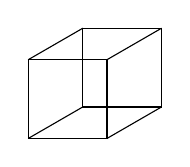
\begin{tikzpicture}[
    x={(1cm,0cm)},
    y={(0cm,1cm)},
    z={(-150:0.8cm)}
]
\draw (0,0,0) -- (1,0,0) -- (1,1,0) -- (0,1,0) -- cycle;
\draw (0,0,1) -- (1,0,1) -- (1,1,1) -- (0,1,1) -- cycle;

\draw (0,0,0) -- (0,0,1);
\draw (1,0,0) -- (1,0,1);
\draw (1,1,0) -- (1,1,1);
\draw (0,1,0) -- (0,1,1);

\end{tikzpicture}
    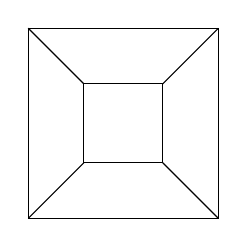
\begin{tikzpicture}
\draw (0,0) --(1,0) -- (1,1) -- (0,1) -- cycle;
\draw (0,0) -- ++(-135:1) coordinate (a);
\draw (1,0) -- ++(-45:1) coordinate (b);
\draw (1,1) -- ++(45:1) coordinate (c);
\draw (0,1) -- ++(135:1) coordinate (d);
\draw (a) -- (b) -- (c) -- (d) -- cycle;
    \end{tikzpicture}
      \caption{A cube and its planar graph.}%
  \label{fig:fullfig}%
\end{marginfigure}

\subsection{Task 1}
Draw the planar graph of an icosahedron. Make sure it has 20 triangles.
\section{From the icosahedron to the football}
We begin with an icosahedron. By subdividing each triangular face into smaller triangles and then projecting the vertices onto a sphere, one obtains a geodesic polyhedron.

One famous example of a polyhedron made from pentagons and hexagons is the football (truncated icosahedron).

Before studying the football, begin with the dodecahedron.

\subsection{Task 2}
How many vertices and edges does the dodecahedron have? How many vertices and edges does the football have? Find a relationship between the number of vertices $V$ and the number of edges $E$ that holds for the football. Does this formula also hold for the dodecahedron? Conjecture a formula that might be true for any polyhedron made entirely from pentagons and hexagons.

Let $F_5$ be the number of pentagonal faces, $F_6$ be the number of hexagonal faces, and $F$ denote the total number of faces.

\subsection{Task 3}

Find $F$ in terms of $F_5$ and $F_6$

\subsection{Task 4}
Each edge belongs to exactly two faces. Use this to derive a formula relating $F_5$, $F_6$, and $E$. 

\section{Euler's formula}

Recall Euler's identity for convex polyhedra:
\begin{equation}
V- E + F= 2
\end{equation}
Use your answer from the previous tasks together with Euler's formula to derive a relationship between $F_5$ and $F_6$. 

What does your result tell you about the number of pentagons in any polyhedron made entirely from pentagons and hexagons?
\begin{marginfigure}
    \begin{tikzpicture}[3d view
]
\coordinate (a1) at (0,1,\phi);
\coordinate (a2) at (0,-1,\phi);
\coordinate (a3) at (0,1,-\phi);
\coordinate (a4) at (0,-1,-\phi);
\coordinate (a5) at (1,\phi,0);
\coordinate (a6) at (-1,\phi,0);
\coordinate (a7) at (1,-\phi,0);
\coordinate (a8) at (-1,-\phi,0);
\coordinate (a9) at (\phi,0,1);
\coordinate (a10) at (\phi,0,-1);
\coordinate (a11) at (-\phi,0,1);
\coordinate (a12) at (-\phi,0,-1);

% \foreach \c in {1,...,12}{
%     \draw (a\c) circle (2pt); 
% }
% \draw[xkcdPurple,very thin] (a1) node[right] {$a_{1}$}-- (a2) node[right] {$a_{2}$}-- (a4) node[right] {$a_{4}$}--(a3)  node[right] {$a_3$} -- cycle;
% \draw[xkcdGreen] (a5)  node[right] {$a_{5}$} -- (a6)  node[right] {$a_{6}$}-- (a8)  node[right] {$a_{8}$}--(a7)  node[right] {$a_{7}$}-- cycle;
% \draw[xkcdBlue] (a9)node[right] {$a_{9}$} -- (a10)node[right] {$a_{10}$} -- (a12)  node[right] {$a_{12}$} --(a11)node[right] {$a_{11}$} -- cycle;
\draw (a1) -- (a2) -- (a9) -- cycle;
\draw (a1) -- (a2) -- (a11) -- cycle;
\draw (a3) -- (a4) -- (a10) -- cycle;
\draw (a3) -- (a4) -- (a12) -- cycle;
\draw (a5) -- (a6) -- (a1) -- cycle;
\draw (a5) -- (a6) -- (a3) -- cycle;
\draw (a7) -- (a8) -- (a2) -- cycle;
\draw (a7) -- (a8) -- (a4) -- cycle;
\draw (a9) -- (a10) -- (a5) -- cycle;
\draw (a9) -- (a10) -- (a7) -- cycle;
\draw (a11) -- (a12) -- (a6) -- cycle;
\draw (a11) -- (a12) -- (a8) -- cycle;
\draw[xkcdMagenta,very thick] (a3) -- (a5) -- (a10) -- cycle;
    \end{tikzpicture}
    \caption{icosahedron}
\end{marginfigure}
Show that every polyhedron whose faces are only pentagons and hexagons must contain exactly 12 pentagons.
\section{Building a GeoSphere}
In this activity, we will construct a \emph{frequency-6} geodesic dome. Start with an icosahedron and divide each edge into 6 equal parts. Joining the new points creates a triangular grid on every face.
\begin{marginfigure}
    \begin{tikzpicture}[3d view,scale=2.5
]
% \clip (a3) rectangle (a9);

\coordinate (a1) at (0,1,\phi);
\coordinate (a2) at (0,-1,\phi);
\coordinate (a3) at (0,1,-\phi);
\coordinate (a4) at (0,-1,-\phi);
\coordinate (a5) at (1,\phi,0);
\coordinate (a6) at (-1,\phi,0);
\coordinate (a7) at (1,-\phi,0);
\coordinate (a8) at (-1,-\phi,0);
\coordinate (a9) at (\phi,0,1);
\coordinate (a10) at (\phi,0,-1);
\coordinate (a11) at (-\phi,0,1);
\coordinate (a12) at (-\phi,0,-1);

% \foreach \c in {1,...,12}{
%     \draw (a\c) circle (2pt); 
% }
% \draw[xkcdPurple,very thin] (a1) node[right] {$a_{1}$}-- (a2) node[right] {$a_{2}$}-- (a4) node[right] {$a_{4}$}--(a3)  node[right] {$a_3$} -- cycle;
% \draw[xkcdGreen] (a5)  node[right] {$a_{5}$} -- (a6)  node[right] {$a_{6}$}-- (a8)  node[right] {$a_{8}$}--(a7)  node[right] {$a_{7}$}-- cycle;
% \draw[xkcdBlue] (a9)node[right] {$a_{9}$} -- (a10)node[right] {$a_{10}$} -- (a12)  node[right] {$a_{12}$} --(a11)node[right] {$a_{11}$} -- cycle;
% \draw (a1) -- (a2) -- (a9) -- cycle;
% \draw (a1) -- (a2) -- (a11) -- cycle;
% \draw (a3) -- (a4) -- (a10) -- cycle;
% \draw (a3) -- (a4) -- (a12) -- cycle;
% \draw (a5) -- (a6) -- (a1) -- cycle;
% \draw (a5) -- (a6) -- (a3) -- cycle;
% \draw (a7) -- (a8) -- (a2) -- cycle;
% \draw (a7) -- (a8) -- (a4) -- cycle;
% \draw (a9) -- (a10) -- (a5) -- cycle;
% \draw (a9) -- (a10) -- (a7) -- cycle;
% \draw (a11) -- (a12) -- (a6) -- cycle;
% \draw (a11) -- (a12) -- (a8) -- cycle;
\draw[xkcdMagenta,very thick] (a3)  -- (a5)  -- (a10)  -- cycle;
\foreach \s in {1/6,1/3,1/2,2/3,5/6}{
    \draw ($ (a3)!\s!(a5) $) -- ($ (a10)!\s!(a5) $);
    \draw ($ (a3)!\s!(a10) $) -- ($ (a5)!\s!(a10) $);
    \draw ($ (a10)!\s!(a3) $) -- ($ (a5)!\s!(a3) $);
}
    \end{tikzpicture}
    \caption{One triangular face of the icosahedron subdivided into smaller triangles.}
\end{marginfigure}
\subsection{Task 5}
After subdividing each edge into 6 equal parts, how many small triangles does each original triangular face contain?

Around each original vertex of the icosahedron, five small triangles meet, giving rise to a pentagon. Around every new interior vertex, six small triangles meet, giving rise to a hexagon.

\subsection{Task 6}
How many pentagons and how many hexagons does this frequency-6 construction produce?

We will build the geosphere using bamboo sticks. Each edge of the final structure is formed by two bamboo sticks. Each bamboo stick is marked with a letter label. Figure~\ref{fig:schema} shows the labelling scheme\nocite{website:ccl}. Use these labels as a guide while weaving the bamboo sticks together to assemble the geosphere.

\begin{figure}
    \begin{tikzpicture}[3d view,scale=5
]
% \clip (a3) rectangle (a9);

\coordinate (a1) at (0,1,\phi);
\coordinate (a2) at (0,-1,\phi);
\coordinate (a3) at (0,1,-\phi);
\coordinate (a4) at (0,-1,-\phi);
\coordinate (a5) at (1,\phi,0);
\coordinate (a6) at (-1,\phi,0);
\coordinate (a7) at (1,-\phi,0);
\coordinate (a8) at (-1,-\phi,0);
\coordinate (a9) at (\phi,0,1);
\coordinate (a10) at (\phi,0,-1);
\coordinate (a11) at (-\phi,0,1);
\coordinate (a12) at (-\phi,0,-1);

% \foreach \c in {1,...,12}{
%     \draw (a\c) circle (2pt); 
% }
% \draw[xkcdPurple,very thin] (a1) node[right] {$a_{1}$}-- (a2) node[right] {$a_{2}$}-- (a4) node[right] {$a_{4}$}--(a3)  node[right] {$a_3$} -- cycle;
% \draw[xkcdGreen] (a5)  node[right] {$a_{5}$} -- (a6)  node[right] {$a_{6}$}-- (a8)  node[right] {$a_{8}$}--(a7)  node[right] {$a_{7}$}-- cycle;
% \draw[xkcdBlue] (a9)node[right] {$a_{9}$} -- (a10)node[right] {$a_{10}$} -- (a12)  node[right] {$a_{12}$} --(a11)node[right] {$a_{11}$} -- cycle;
% \draw (a1) -- (a2) -- (a9) -- cycle;
% \draw (a1) -- (a2) -- (a11) -- cycle;
% \draw (a3) -- (a4) -- (a10) -- cycle;
% \draw (a3) -- (a4) -- (a12) -- cycle;
% \draw (a5) -- (a6) -- (a1) -- cycle;
% \draw (a5) -- (a6) -- (a3) -- cycle;
% \draw (a7) -- (a8) -- (a2) -- cycle;
% \draw (a7) -- (a8) -- (a4) -- cycle;
% \draw (a9) -- (a10) -- (a5) -- cycle;
% \draw (a9) -- (a10) -- (a7) -- cycle;
% \draw (a11) -- (a12) -- (a6) -- cycle;
% \draw (a11) -- (a12) -- (a8) -- cycle;
\draw[xkcdMagenta, dashed] (a3)  -- (a5)  -- (a10)  -- cycle;
\foreach \s in {1/6,1/3,1/2,2/3,5/6}{
    \draw[very thin, dashed] ($ (a3)!\s!(a5) $) -- ($ (a10)!\s!(a5) $);
    \draw[very thin, dashed] ($ (a3)!\s!(a10) $) -- ($ (a5)!\s!(a10) $);
    \draw[very thin, dashed] ($ (a10)!\s!(a3) $) -- ($ (a5)!\s!(a3) $);
}
\draw ($ (a3)!{5/6}!(a5) $) -- node[midway, above] {$A$} ($ (a10)!{5/6}!(a5) $)--node[midway, right] {$A$} ($ (a9)!{5/6}!(a5) $)-- node[midway, above] {$A$} ($ (a1)!{5/6}!(a5) $)-- node[midway, above] {$A$} ($ (a6)!{5/6}!(a5) $) -- node[midway, left] {$A$} cycle;

\draw ($ (a3)!{1/6}!(a5) $) -- node[midway, above] {$A$} ($ (a3)!{1/6}!(a10) $)--node[midway, right] {$A$} ($ (a3)!{1/6}!(a4) $)-- node[midway, below] {$A$} ($ (a3)!{1/6}!(a12) $)-- node[midway, left] {$A$} ($ (a3)!{1/6}!(a6) $) -- node[midway, above] {$A$} cycle;

\draw ($ (a10)!{1/6}!(a5) $) -- node[midway, above] {$A$} ($ (a10)!{1/6}!(a9) $)--node[midway, right] {$A$} ($ (a10)!{1/6}!(a7) $)-- node[midway, right] {$A$} ($ (a10)!{1/6}!(a4) $)-- node[midway, below] {$A$} ($ (a10)!{1/6}!(a3) $) -- node[midway, left] {$A$} cycle;

\draw ($ (a3)!{5/6}!(a5) $) -- ($ (a10)!{5/6}!(a5) $) -- node[midway, right] {$B$}  ($ (a10)!{2/3}!(a5) $) -- node[midway, right] {$C$} ($ ($ (a3)!{1/2}!(a5) $)!{2/3}!($ (a10)!{1/2}!(a5) $) $)-- node[midway, below] {$D$} ($ ($ (a3)!{1/2}!(a5) $)!{1/3}!($ (a10)!{1/2}!(a5) $) $)-- node[midway, left] {$C$} ($ (a3)!{2/3}!(a5) $) -- node[midway, left] {$B$} cycle;

\draw ($ (a10)!{5/6}!(a3) $) -- ($ (a5)!{5/6}!(a3) $) -- node[midway, left] {$B$}  ($ (a5)!{2/3}!(a3) $) -- node[midway, above] {$C$} ($ ($ (a10)!{1/2}!(a3) $)!{2/3}!($ (a5)!{1/2}!(a3) $) $)-- node[midway, right] {$D$} ($ ($ (a10)!{1/2}!(a3) $)!{1/3}!($ (a5)!{1/2}!(a3) $) $)-- node[midway, right] {$C$} ($ (a10)!{2/3}!(a3) $) -- node[midway, below] {$B$} cycle;

\draw ($ (a5)!{5/6}!(a10) $) -- ($ (a3)!{5/6}!(a10) $) -- node[midway, below] {$B$}  ($ (a3)!{2/3}!(a10) $) -- node[midway, right] {$C$} ($ ($ (a5)!{1/2}!(a10) $)!{2/3}!($ (a3)!{1/2}!(a10) $) $)-- node[midway, right] {$D$} ($ ($ (a5)!{1/2}!(a10) $)!{1/3}!($ (a3)!{1/2}!(a10) $) $)-- node[midway, above] {$C$} ($ (a5)!{2/3}!(a10) $) -- node[midway, above] {$B$} cycle;

\draw  ($ ($ (a3)!{1/2}!(a5) $)!{1/3}!($ (a10)!{1/2}!(a5) $) $)-- node[midway, left] {$E$} ($ ($ (a10)!{1/2}!(a3) $)!{2/3}!($ (a5)!{1/2}!(a3) $) $);
\draw  ($ ($ (a3)!{1/2}!(a5) $)!{2/3}!($ (a10)!{1/2}!(a5) $) $)-- node[midway, right] {$E$} ($ ($ (a5)!{1/2}!(a10) $)!{1/3}!($ (a3)!{1/2}!(a10) $) $);

\draw ($ ($ (a10)!{1/2}!(a3) $)!{1/3}!($ (a5)!{1/2}!(a3) $) $)--node[midway,below] {$E$} ($ ($ (a5)!{1/2}!(a10) $)!{2/3}!($ (a3)!{1/2}!(a10) $) $);

    \end{tikzpicture}
    \caption{Schema}
    \makeatletter
\typeout{CURRENTLABEL=\@currentlabel}
\makeatother
        \label{fig:schema}
\end{figure}

Compare the geosphere you have built with the football studied earlier. What similarities and differences do you notice?
\bibliography{geoSphere}
\bibliographystyle{plainnat}
\end{document}